\chapter{Background e Stato dell'Arte}

L'evoluzione del panorama delle minacce informatiche ha reso indispensabile lo sviluppo di tecniche e strumenti sempre più sofisticati per l'analisi forense digitale. Questo capitolo fornisce le basi teoriche necessarie per comprendere il contesto in cui si inserisce il presente lavoro, esplorando i concetti fondamentali del Digital Forensics and Incident Response (DFIR), con particolare attenzione all'analisi della memoria volatile. Verranno inoltre esaminati i principali framework esistenti, con focus su Volatility e YARA, evidenziando le limitazioni che motivano le espansioni proposte in questa tesi.

\section{Digital Forensics e Incident Response (DFIR)}

\subsection{Definizione e principi fondamentali}

Il Digital Forensics and Incident Response (DFIR) rappresenta la convergenza di due discipline complementari che, insieme, formano il nucleo delle capacità di risposta alle minacce cyber moderne. Il termine DFIR è stato coniato per riflettere la natura interconnessa di queste attività nel contesto operativo reale.

La Digital Forensics si fonda su quattro principi scientifici fondamentali che ne garantiscono il rigore metodologico \cite{kent2006}. La preservazione dell'evidenza assicura che i dati non vengano alterati durante l'acquisizione e l'analisi, mentre la chain of custody documenta ogni passaggio per mantenere l'ammissibilità legale delle prove. A questi si aggiungono la ripetibilità delle analisi, che devono produrre risultati consistenti, e la documentazione completa di ogni azione intrapresa, elementi che insieme formano il framework metodologico codificato negli standard internazionali come ISO/IEC 27037:2012 \cite{iso27037}.

Questi principi sono ulteriormente rafforzati dalle linee guida SWGDE \cite{swgde2022} che stabiliscono best practices specifiche per la preservazione di evidenze volatili come pagine web, social media e comunicazioni cloud-based, riflettendo l'evoluzione delle fonti di evidenza nell'era digitale moderna.

L'Incident Response si concentra invece sulla gestione operativa degli incidenti di sicurezza con l'obiettivo di minimizzare l'impatto e ripristinare le operazioni normali nel minor tempo possibile. Il SANS Institute la definisce come "un approccio organizzato per affrontare e gestire le conseguenze di una violazione della sicurezza o di un attacco informatico" \cite{sans2023}.

La fusione di queste discipline nel DFIR riconosce che, nel mondo reale, l'analisi forense e la risposta agli incidenti sono attività inseparabili. Durante un incidente attivo, i responder devono bilanciare molteplici esigenze contrastanti: contenere la minaccia mentre preservano le evidenze, analizzare i sistemi compromessi senza interrompere le operazioni critiche, e trovare il giusto equilibrio tra la necessità di un'indagine approfondita e l'urgenza del ripristino operativo.

\subsection{Il processo DFIR}

Il processo DFIR segue un approccio metodologico articolato in sei fasi distinte, come definito dal framework NIST SP 800-61 \cite{cichonski2012}. Sebbene questa struttura fornisca un modello logico di riferimento, nella pratica operativa le fasi si sovrappongono frequentemente e richiedono un approccio iterativo.

\begin{figure}[H]
    \centering
    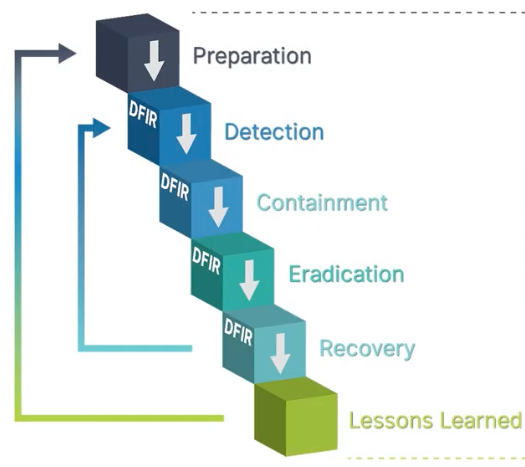
\includegraphics[width=0.6\linewidth]{images/stato-arte/digital-forensics-incident-response-plan-flow.png}
\end{figure}

La preparazione rappresenta il fondamento dell'intero processo, determinando la differenza tra una risposta efficace e una gestione caotica. Questa fase richiede lo sviluppo preventivo di playbook e procedure operative standard, supportati da un'infrastruttura tecnologica adeguata e training continuo del personale. L'identificazione inizia con l'analisi degli alert provenienti dai sistemi di sicurezza, seguita da un processo di triage che distingue i falsi positivi dalle minacce concrete. Il contenimento diventa poi prioritario per limitare la propagazione del danno attraverso azioni immediate di isolamento e misure sostenibili a lungo termine, sempre preservando le evidenze forensi.

L'eradicazione richiede un approccio sistematico che va oltre la rimozione degli artefatti visibili, identificando tutti i componenti malevoli, incluse backdoor e meccanismi di persistenza nascosti. Il recupero rappresenta una fase delicata dove la ricostruzione deve partire da backup verificati, accompagnata da monitoraggio intensificato. Infine, la fase di lessons learned trasforma ogni incidente in un'opportunità di miglioramento attraverso documentazione dettagliata e analisi critica.

Il DFIR è ormai essenziale nella cybersecurity moderna sia per fronteggiare minacce avanzate come APT e ransomware, sia per rispondere a requisiti normativi stringenti come il GDPR \cite{gdpr2016} che impone notifica entro 72 ore, la direttiva NIS2 \cite{nis2_2022} per operatori essenziali, e il DORA \cite{dora2022} per il settore finanziario. Con il tempo medio di permanenza degli attaccanti sceso a 16 giorni \cite{mandiant2023}, la capacità di risposta rapida ed efficace diventa critica.

\section{Memory Forensics}

\subsection{La memoria volatile come fonte di evidenze}

La memoria volatile, principalmente la RAM, rappresenta lo stato "vivo" di un sistema informatico catturando informazioni effimere ma fondamentali che rivelano con precisione cosa stava accadendo al momento dell'acquisizione \cite{ligh2014}. A differenza dello storage persistente, la memoria offre una finestra unica sui processi in esecuzione, le connessioni di rete attive, e i dati temporaneamente decifrati.

L'architettura della memoria segue una gerarchia complessa che parte dai registri CPU ultra-veloci ma minuscoli, attraversa le cache L1-L3 progressivamente più capienti, e culmina nella RAM principale che costituisce l'area di lavoro del sistema. Questa contiene lo spazio kernel con le strutture critiche del sistema operativo, lo spazio utente dove risiedono processi e applicazioni, la pool memory per allocazioni dinamiche, e la page cache con i dati dei file recenti.

La gestione della memoria virtuale aggiunge complessità ma anche opportunità investigative. Ogni processo opera in uno spazio di indirizzamento isolato, con pagine virtuali mappate dinamicamente su frame fisici attraverso page tables e translation lookaside buffers. Per l'analista forense, ricostruire questi mapping è essenziale per interpretare correttamente il contenuto della memoria \cite{case2017}.

\subsection{Artefatti recuperabili e vantaggi dell'analisi}

La memoria volatile conserva artefatti unici non reperibili altrove. I processi e thread rivelano l'intera lista dei processi, inclusi quelli nascosti da rootkit, con argomenti command line, variabili d'ambiente, handle aperti, stack e heap contenenti tracce dell'esecuzione. Le informazioni di rete mostrano connessioni TCP/UDP attive, socket in ascolto che potrebbero nascondere backdoor, cache DNS e buffer di pacchetti.

Particolarmente critici sono gli artefatti di sicurezza: token di autenticazione e chiavi crittografiche temporaneamente in chiaro, certificati SSL/TLS, ticket Kerberos, hash NTLM e password di applicazioni. Le evidenze di malware includono codice iniettato in processi legittimi, API hooks, driver kernel malevoli, payload cifrati decriptati solo a runtime, e comunicazioni C\&C. Le tracce di attività utente comprendono clipboard, titoli di finestre, cronologia comandi, documenti in editing e chat in chiaro.

L'analisi della memoria offre vantaggi unici rispetto all'analisi del disco. Garantisce visibilità su minacce fileless e tecniche living-off-the-land che non lasciano tracce su disco. Permette l'accesso a dati normalmente cifrati, osservabili in chiaro durante l'esecuzione. Fornisce una visione runtime completa con processi, connessioni e allocazioni dinamiche, con una timeline difficilmente falsificabile. Inoltre, bypassa molte contromisure anti-forensi poiché modifiche ai file o cancellazioni secure non influenzano le strutture in RAM.

\section{Framework e Strumenti per l'Analisi della Memoria}

\subsection{Volatility Framework}

Volatility \cite{volatility2024} rappresenta lo standard de facto per l'analisi forense della memoria dal suo rilascio nel 2007. Creato inizialmente da Aaron Walters per democratizzare l'accesso a tecniche precedentemente riservate a poche agenzie, il framework si è evoluto attraverso tre versioni maggiori. Volatility 2.0 (2011) introdusse l'architettura plugin-based che ne permise l'espansione da parte della community. Volatility 3 (2019) rappresentò una riscrittura completa in Python 3, risolvendo limitazioni architetturali accumulate e migliorando significativamente le performance.

L'architettura di Volatility 3 si basa su componenti modulari elegantemente integrati. Il Framework Core orchestra configurazione ed esecuzione, mentre le Symbol Tables permettono di interpretare le strutture dati specifiche di ogni versione di sistema operativo. Gli Address Spaces forniscono astrazione per diversi formats di dump, i Plugins implementano la logica di estrazione degli artefatti, e i Renderers gestiscono l'output in formati multipli.

Il framework offre oltre 100 plugin che coprono ogni aspetto dell'analisi. Per l'analisi dei processi, \texttt{pstree} visualizza relazioni gerarchiche evidenziando anomalie parent-child spesso indicative di injection, mentre \texttt{psscan} esegue scansioni euristiche per scoprire processi nascosti da rootkit. L'estrazione delle command line con \texttt{cmdline} rivela gli obiettivi degli attaccanti, e l'analisi di DLL e handle fornisce insight sulle risorse manipolate.

Per l'analisi di rete, \texttt{netscan} (ottimizzato per Windows Vista+) fornisce una visione comprensiva delle connessioni, evoluzione dei precedenti plugin per sistemi legacy. La detection di malware si avvale di \texttt{malfind} che implementa euristiche sofisticate per identificare code injection cercando pagine eseguibili non mappate a file - combinazione altamente sospetta. Plugin complementari come \texttt{hollowfind} specializzano la ricerca verso process hollowing, mentre l'analisi dei callback kernel può rivelare rootkit a livello kernel.

\subsection{YARA}

YARA \cite{yara2024}, creato da Victor M. Alvarez presso VirusTotal nel 2008, è diventato lo standard per pattern matching e classificazione di malware. Il suo successo deriva dalla capacità di descrivere famiglie di malware attraverso regole basate su caratteristiche testuali o binarie, applicabili a file, processi o dump di memoria.

La sintassi YARA bilancia espressività e semplicità. Una regola tipica contiene tre sezioni: \textbf{meta} con metadati descrittivi, \textbf{strings} che definisce i pattern da cercare (stringhe, hex, regex), e \textbf{condition} che specifica la logica booleana per il matching. 

\begin{minted}[
    breaklines,
    frame=lines,
    framesep=2mm,
    baselinestretch=1.2,
    fontsize=\small,
    linenos
]{c}
rule ExampleRule {
    meta:
        author = "Security Researcher"
        description = "Detects Example Malware"
        date = "2024-01-01" 
    strings:
        $text_string = "malicious_function"
        $hex_string = { 6A 40 68 00 30 00 00 6A 14 8D }
        $regex = /\w+\.exe/
    condition:
        any of them
}
\end{minted}

La flessibilità delle condizioni permette logiche detection estremamente sofisticate utilizzando operatori logici, contatori, offset e funzioni built-in. Le condizioni possono essere semplici ("any of them") o complesse, combinando multipli criteri per ridurre i falsi positivi e aumentare l'accuratezza del rilevamento.

Quando applicato alla memoria, YARA trasforma le capacità investigative. Eccelle nell'identificare malware che esistono solo runtime - shellcode iniettato in processi legittimi, DLL reflective che non toccano disco, payload che si materializzano solo post-exploitation. Durante il threat hunting, YARA cerca stringhe uniche di famiglie malware specifiche, pattern di comunicazione C2, o artefatti di tool post-exploitation come Cobalt Strike.

La vera potenza emerge nel rilevamento di tecniche di evasione. YARA può identificare pattern lasciati da process hollowing dove processi legittimi vengono svuotati e riempiti con codice malevolo, riconoscere API hooks sospetti, o pattern di allocazione memoria che tradiscono injection avanzate. Ogni tecnica di evasione, per quanto sofisticata, lascia inevitabilmente una firma che YARA può essere addestrata a riconoscere.

Volatility integra nativamente YARA attraverso il plugin \texttt{yarascan}, che non si limita a segnalare match ma fornisce ricco contesto forense: offset di memoria per correlazioni, processo proprietario per attribuzione, permessi della pagina (RWX spesso indica injection), e dump del contenuto circostante per analisi manuale approfondita.

\subsection{Limitazioni degli approcci attuali}

Nonostante la maturità degli strumenti disponibili, l'adozione della memory forensics rimane limitata da barriere sistemiche che ne impediscono il pieno potenziale.

La complessità tecnica costituisce l'ostacolo principale. L'analisi efficace richiede non solo competenza sui tool ma comprensione profonda di architetture OS, gestione memoria, e tecniche anti-forensics. Interpretare i risultati necessita esperienza per distinguere comportamenti normali da anomalie in contesti diversi. La necessità di scripting per automazione esclude personale non programmatore, creando un collo di bottiglia nelle capacità investigative delle organizzazioni.

L'interfaccia command-line di Volatility, per quanto potente per utenti esperti, rallenta significativamente il processo di triage iniziale quando ogni minuto conta. L'output testuale non strutturato richiede post-processing manuale intensivo per identificare informazioni rilevanti, mentre l'integrazione limitata con YARA impedisce ricerche complesse basate su pattern comportamentali. L'assenza di funzionalità collaborative native rappresenta un ulteriore ostacolo in contesti dove il lavoro di team è essenziale.

Gli strumenti commerciali come Magnet AXIOM e Mandiant Redline, pur offrendo interfacce più intuitive, presentano limitazioni critiche in contesti competitivi. I modelli di licensing restrittivi limitano l'accesso simultaneo necessario per team numerosi, mentre le capacità di customizzazione limitate impediscono l'implementazione rapida di nuove tecniche analitiche richieste da scenari in evoluzione.

L'assenza di standard condivisi e l'incompatibilità tra strumenti creano inefficienze sistemiche che se amplificano sotto pressione temporale. La necessità di utilizzare tool multipli per coprire l'intero spettro di requisiti introduce overhead significativo nel trasferimento di dati e contesto. I problemi di scalabilità emergono in scenari enterprise dove incidenti coinvolgono centinaia di endpoint. L'analisi sequenziale di dump multipli diventa proibitiva senza parallelizzazione nativa.

L'integrazione limitata con l'ecosistema di sicurezza riduce il valore operativo. Threat intelligence feeds non si integrano nativamente, la correlazione con logs e network traffic è manuale, export verso piattaforme avanzate richiede trasformazioni complesse, e API limitate impediscono automazione enterprise-grade.

Le limitazioni identificate negli approcci tradizionali hanno creato lo spazio per soluzioni innovative come VolWeb \cite{volweb2024}, che si propone di colmare il gap tra la potenza analitica di Volatility e l'accessibilità richiesta dai moderni team di sicurezza. Il prossimo capitolo esamina in dettaglio come VolWeb affronta queste sfide attraverso la sua architettura web-based e l'approccio user-centric.